\subsection{Descrizione generale}
	Durante la fase di progettazione la struttura del prodotto è stata modellata in quattro componenti distinte:
	\begin{itemize}
		\item \textbf{server}: motore di calcolo che coordina le unità e genera le informazioni per la UI; viene modellato seguendo la \textit{layered architecture};
		\item \textbf{interfaccia grafica}: mostra la mappa e permette di gestire le unità e gli utenti; viene modellata seguendo il \textit{MVVM};
		\item \textbf{unità}: si occupa di simulare il comportamento di un'unità all'interno dell'ambiente; viene modellata seguendo la \textit{hexagonal architecture};
		\item \textbf{sensori}: si occupa di simulare il comportamento dei sensori delle unità all'interno dell'ambiente; non viene modellato secondo una architettura specifica poiché triviale.
	\end{itemize}
	La UI e l'unità comunicano con il server tramite l'uso di \glock{WebSocket} e lo scambio di messaggi \glock{JSON}. Il server, quindi, conoscendo la posizione di tutte le unità e ostacoli, genera il percorso migliore, lo comunica alle unità richiedenti e aggiorna la mappa informando l'interfaccia grafica.\\

\subsection{Architettura del server}
	Il pattern architetturale applicato alla componente server è la \textit{Layered Architecture}. \\
	Si è scelto tale pattern in quanto la componente server risulta troppo complessa per essere destrutturata dovendo gestire i servizi di: anagrafica unità, anagrafica utente, gestione mappa, calcolo percorsi unità e gestione delle interfacce grafiche.\\
	Di seguito viene illustrato il diagramma dei package. Si noti che le dipendenze procedono in un'unica direzione senza creare cicli. Si noti, inoltre, che il sistema dipende dalla classe \textbf{Position} in ogni suo punto in quanto, trattando problematiche legate al movimento di un'unità in una griglia, avere un tipo di dato che rappresenti due coordinate cartesiane risulta particolarmente utile.

	\begin{figure}[H]
		\centering
		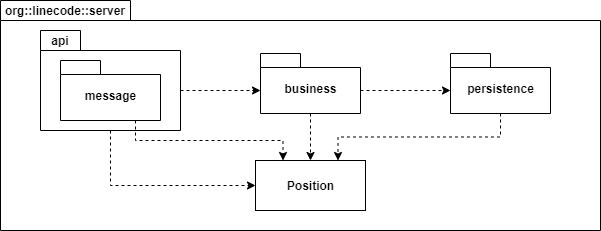
\includegraphics[width=12cm]{img/server_package.png}
		\caption{Server - Diagramma dei package}
	\end{figure}
	
	\begin{figure}[H]
		\centering
		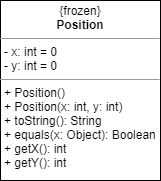
\includegraphics[width=4cm]{img/class_position.png}
		\caption{Server - Classe Position}
	\end{figure}

	\subsubsection{Messaggi}
		È stato stabilito un formato standard di messaggi da e per UI e unità. Tali messaggi sono rappresentati come classi \glock{Java} e verranno scambiati con le altre componenti del prodotto in seguito alla loro serializzazione e deserializzazione in formato \glock{JSON}.\\
		Tutte le classi (vedi figure 3 e 4) estendono la classe astratta Message.
	
		\begin{landscape}
			\begin{figure}[]
				\centering
				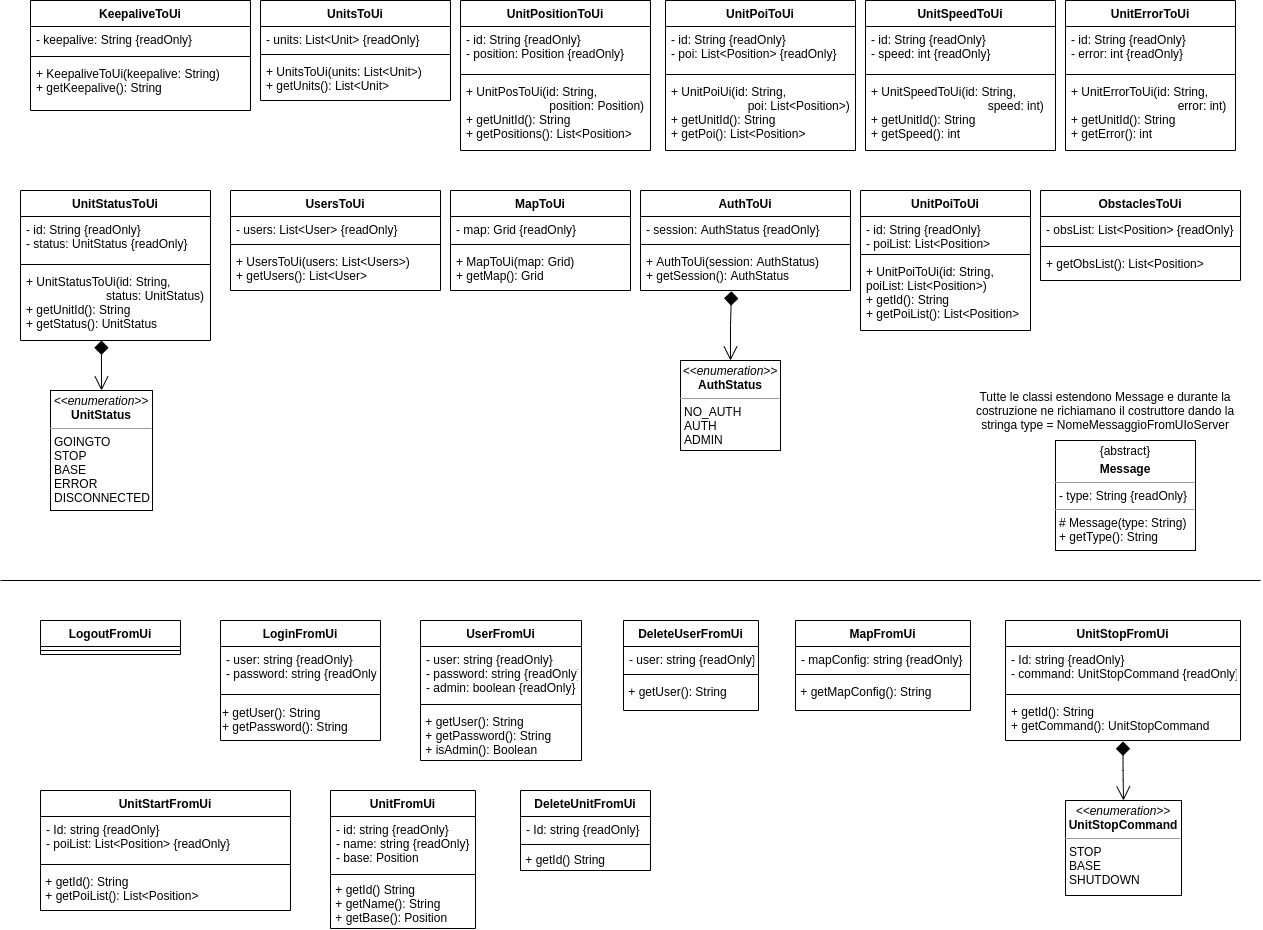
\includegraphics[width=23cm]{img/server_from_to_ui.png}
				\caption{Server - Messaggi da e per l'interfaccia}
			\end{figure}
		\end{landscape}
		\begin{landscape}

			\begin{figure}[H]
				\centering
				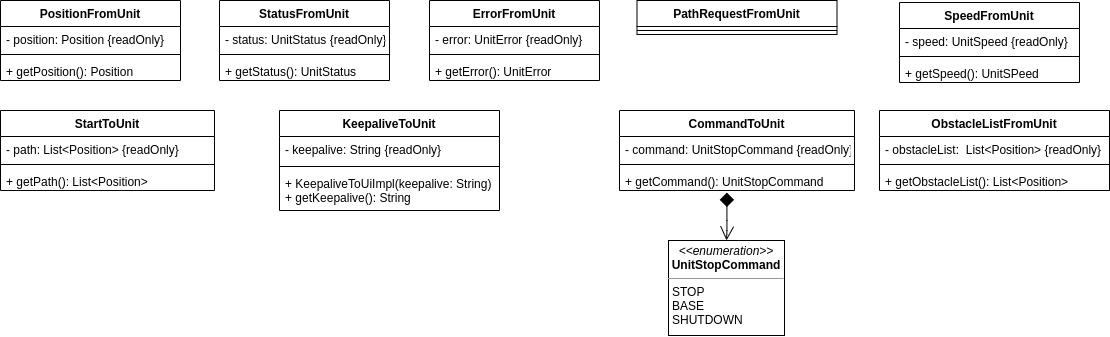
\includegraphics[width=22cm]{img/server_from_to_unit.png}
				\caption{Server - Messaggi da e per l'unità}
			\end{figure}
		\end{landscape}

	\subsubsection{API layer}
		Qui troviamo i metodi che permettono la gestione della connessione alle altre componenti del sistema, e quindi anche l'invio e la ricezione di messaggi mediante opportune serializzazioni e deserializzazioni. Il tutto viene gestito dallo standard JRS 356 per i \glock{WebSocket} e da \glock{Jackson} per la (de)serializzazione.

	\subsubsection{Business layer}
		Qui troviamo la logica per l'elaborazione dei dati. Le informazioni scendono in questo layer tramite chiamata a funzione da parte dell'API layer su opportune interfacce. I prodotti dell'elaborazione vengono riportati nel layer superiore tramite oggetto ritornato dai metodi oppure, quando l'oggetto chiamante non è lo stesso che deve ricevere quanto ritornato, tramite l'emissione di opportuni segnali che verranno intercettati dal layer sovrastante secondo una logica \glock{signal/slot} simile alla libreria grafica \glock{Qt} fornita dalla libreria \glock{Sig4j}. Lo slot viene consegnato tramite chiamata a funzione dall'API layer alla costruzione dell'istanza Endpoint in modo che possa avvenire la connessione fra segnale e slot. In tal modo viene messo in atto un sistema di scambio dei messaggi "dal basso verso l'alto" mantenendo la direzione delle dipendenze in senso contrario.

	\subsubsection{Persistence layer}
		Qui troviamo le classi che permettono al Business layer di relazionarsi con il database indipendentemente dall'implementazione dello stesso grazie all'uso di opportune interfacce.

		\begin{landscape}
			\begin{figure}[h!]
				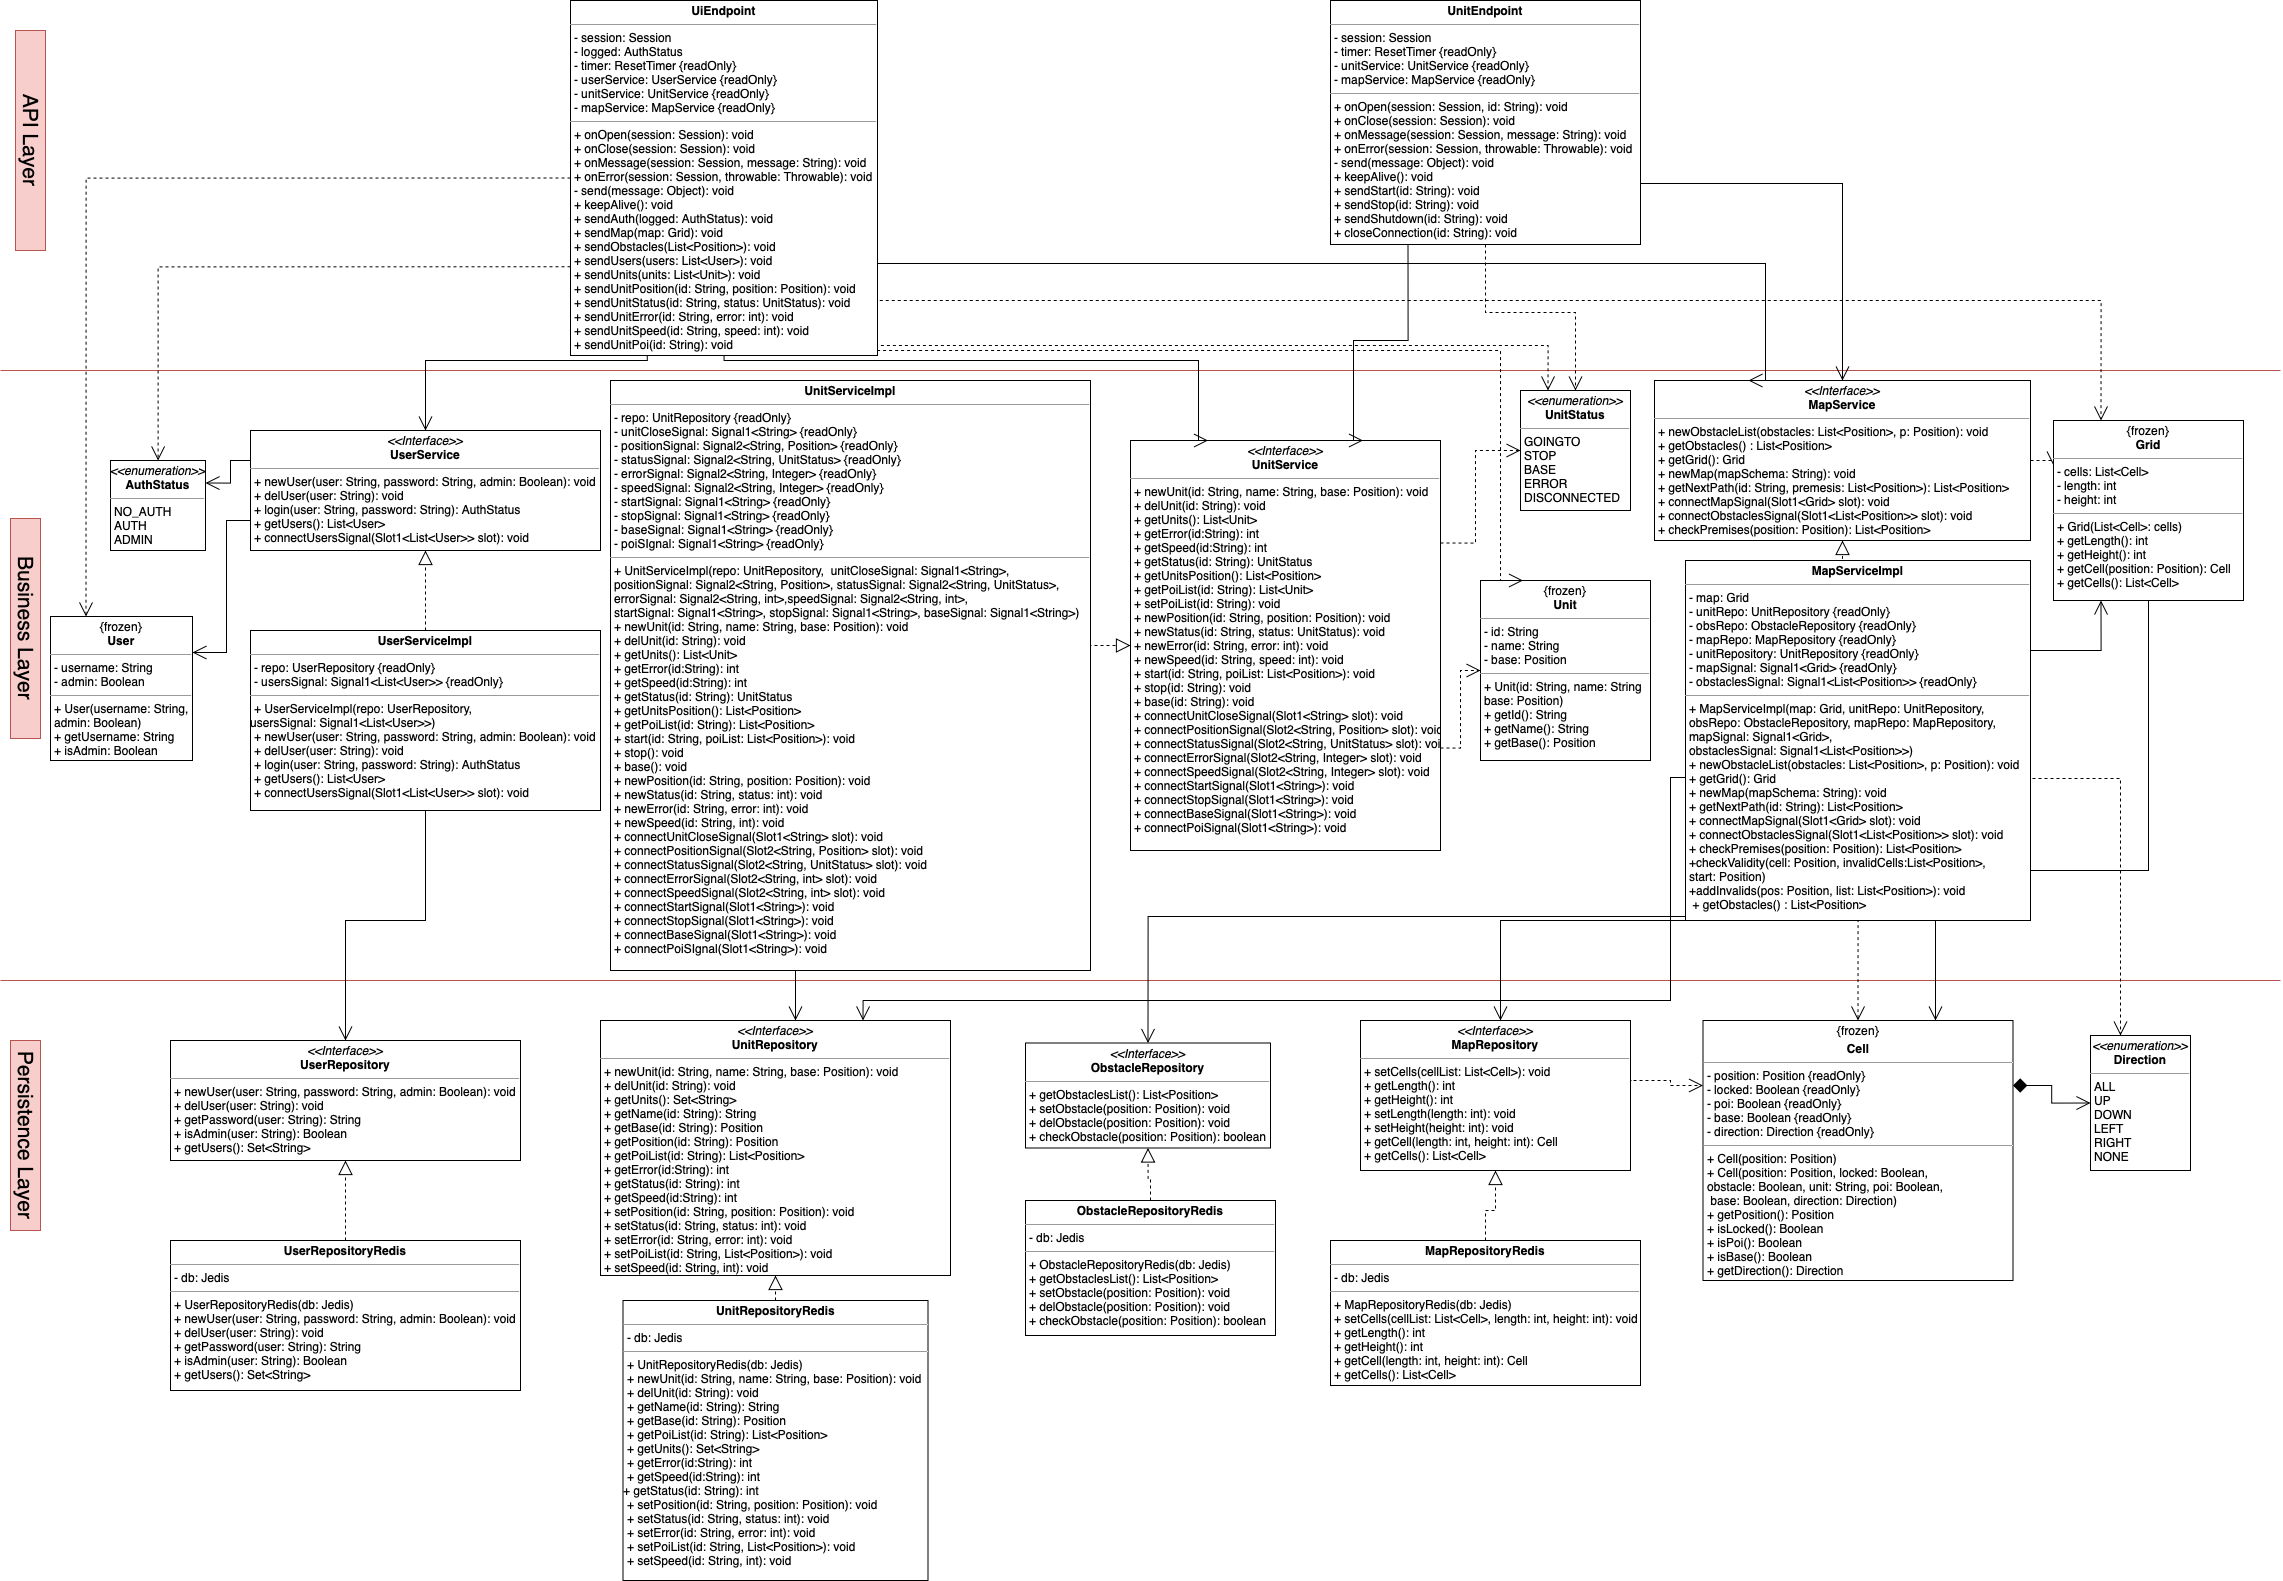
\includegraphics[width=26cm]{img/server_classi.png}
				\caption{Server - Diagramma delle classi}
			\end{figure}
		\end{landscape}
	
	\subsubsection{Database layer}
		Per garantire le migliori performance al sistema e vista la quantità non eccessiva di dati, si è scelto \glock{Redis} come database essendo esso \glock{in-memory}. Non esistono diagrammi standard per rappresentarne la struttura dunque verranno elencate le strutture dati nella tabella seguente:
		
		\begin{table} [h!]
			\rowcolors{2}{gray!25}{gray!6}
			\begin{center}
				\begin{tabular} { m{6cm} m{4cm} m{2cm} m{4cm}}
					\rowcolor{lightgray}
					\textbf{Descrizione} & \textbf{Key} & \textbf{Tipo} & \textbf{Valori / Campi Dati}\\
					id delle unità & unit & SET & \\
					dati e anagrafica delle unità & unit:[id\_unit] & HASH & 
						\begin{itemize}
							\item name
							\item base\_x
							\item base\_y
							\item position\_x
							\item position\_y
							\item status
							\item error
							\item speed
						\end{itemize}\\
					coordinate \glock{POI} da raggiungere per una specifica unità & poi:[id\_unit] & LIST & [coord\_x]:[coord\_y]\\
					username degli user & user & SET & \\
					anagrafica degli user & user:[username] & HASH & 
						\begin{itemize}
							\item password
							\item admin
						\end{itemize}\\
					lunghezza tabella (asse x) & length & STRING & \\
					altezza tabella (asse y) & height & STRING & \\
					dati delle celle della mappa & cell:[coord\_x]:[coord\_y] & HASH & 
						\begin{itemize}
							\item locked
							\item base
							\item direction
							\item poi
						\end{itemize}\\
					id degli ostacoli (intero incrementale) con posizione & obs:[id\_obs] & LIST & [coord\_x]:[coord\_y]\\
				\end{tabular}
			\end{center}
		\end{table}
	
		\newpage
	
		\begin{landscape}
			\subsubsection{Diagrammi di sequenza}
			Il seguente diagramma rappresenta il caso in cui l'interfaccia grafica invii al server una lista di \glock{POI}, che l'unità deve raggiungere.\\
			\begin{figure}[H]
				\centering
				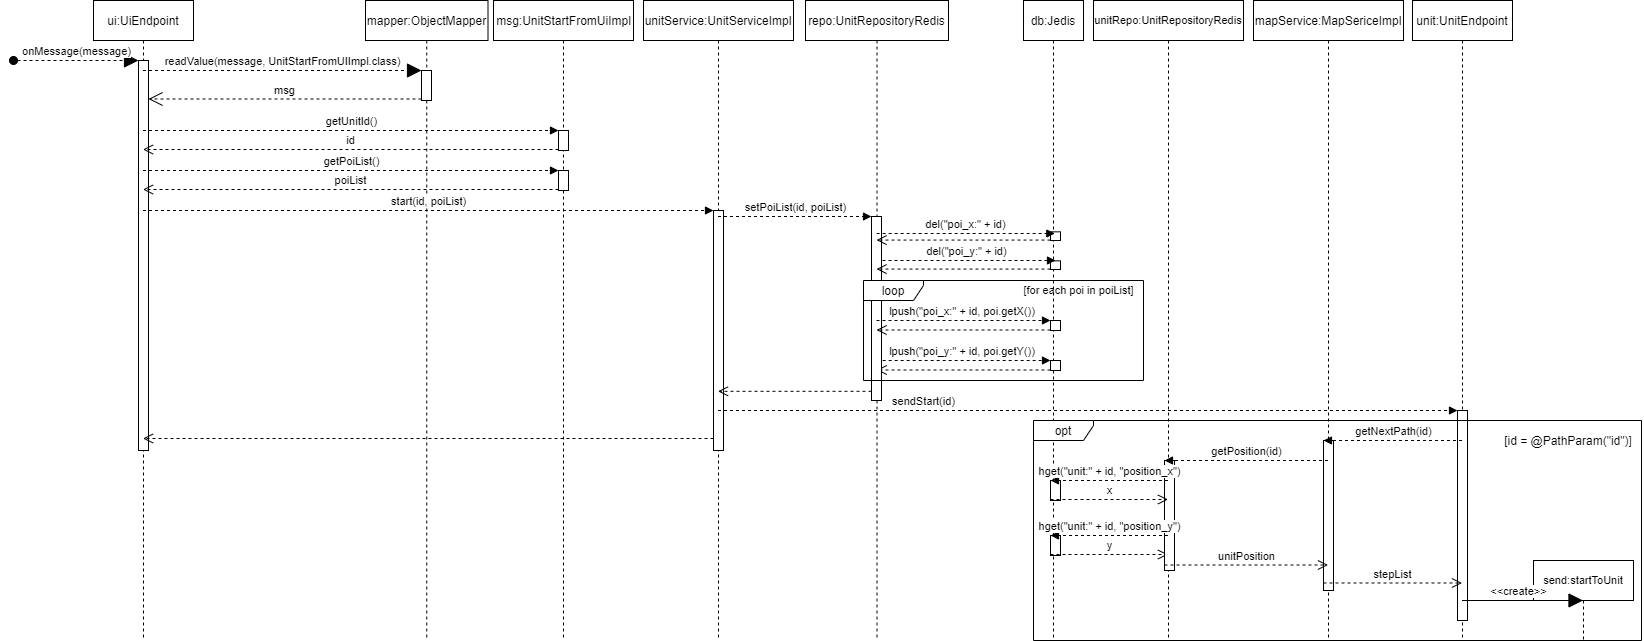
\includegraphics[width=25.7cm]{img/server_seq1.png}
				\caption{Server - UI invia una lista di \glock{POI} che l'unità deve raggiungere}
			\end{figure}
		\end{landscape}
		
		\newpage
		
		\begin{landscape}
			Il seguente diagramma rappresenta il caso in cui un utente esegua il login dall'interfaccia grafica.
			\begin{figure}[H]
				\centering
				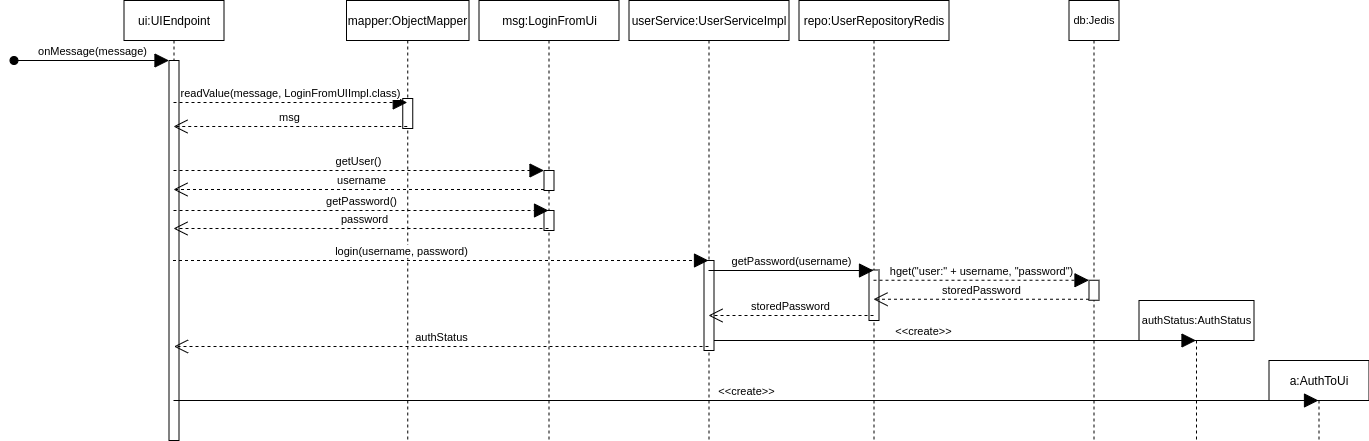
\includegraphics[width=25.7cm]{img/server_seq2.png}
				\caption{Server - Richiesta di login da parte della UI}
			\end{figure}
		\end{landscape}

		\newpage

		\begin{landscape}
			Il seguente diagramma rappresenta il caso in cui un utente elimini un'unità registrata.
			\begin{figure}[H]
				\centering
				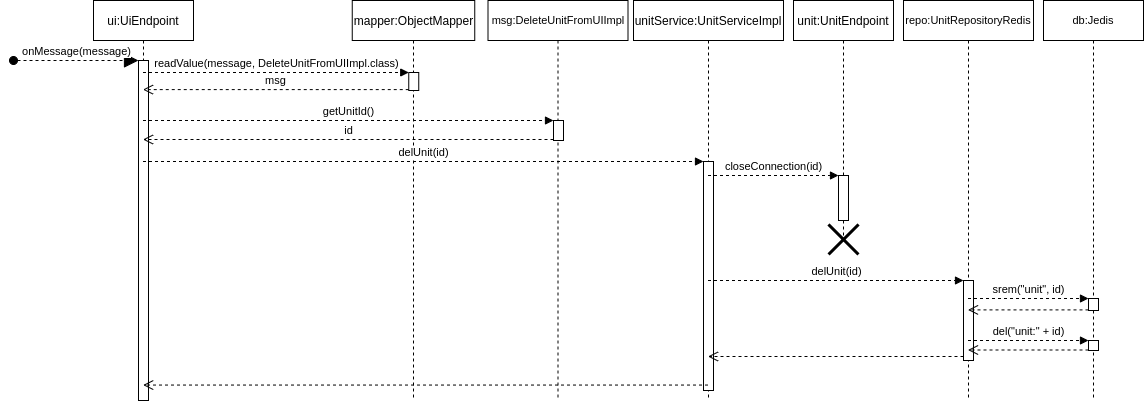
\includegraphics[width=25.7cm]{img/server_seq3.png}
				\caption{Server - UI richiede eliminazione unità}
			\end{figure}
		\end{landscape}
	
\subsection{Architettura dell'interfaccia}
	L'interfaccia grafica è realizzata tramite il framework \glock{Angular}, per questo motivo, il design architetturale utilizzato è il \textit{Model View ViewModel} (\textit{MVVM}) che è intrinseco nel framework stesso. \\
	La comunicazione con il server avviene tramite \glock{WebSocket} ed è dunque asincrona. 
	Inoltre, per garantire l'estensibilità del codice, il servizio \textit{WebSocketService} implementa l'interfaccia \textit{ServerService} che mette a disposizione i metodi per interfacciarsi con il server. In questo modo un cambio di tecnologia, ad esempio passando a richieste \glock{HTTP}, non comporterebbe uno stravolgimento dell'architettura. \\
	Per lo stesso motivo sono previste delle interfacce per rappresentare i vari tipi di messaggi che vengono ricevuti dal server, successivamente implementate per specificarne le caratteristiche. \\
	Ogni componente che fa parte del \textit{ViewModel} rappresenta una funzionalità principale che l'interfaccia mette a disposizione all'utente.\\
	L'aggiornamento dei dati tra gli \glock{Angular Components} ed il \glock{WebSocket} avviene tramite l'uso dei \glock{Subject} (uno per tipo) al'interno di quest'ultimo; indirizzando tali dati  ai componenti che prevedono appositi campi dati per ricevere le informazioni.\\
	\newline
	Di seguito due diagrammi delle classi: il primo per descrivere il legame tra \textit{Model} e \textit{Viewmodel}, con la struttura dei vari \glock{Angular Components}, mentre la parte di \textit{View}; che comprende i templates degli \glock{Angular Components}, non viene qui rappresentata perché la struttura del codice è \glock{HTML}.
	Il secondo, invece, rappresenta i messaggi che vengono inviati e ricevuti dal server.
	\newpage
	
	\begin{landscape}
		\begin{figure}[h!]
			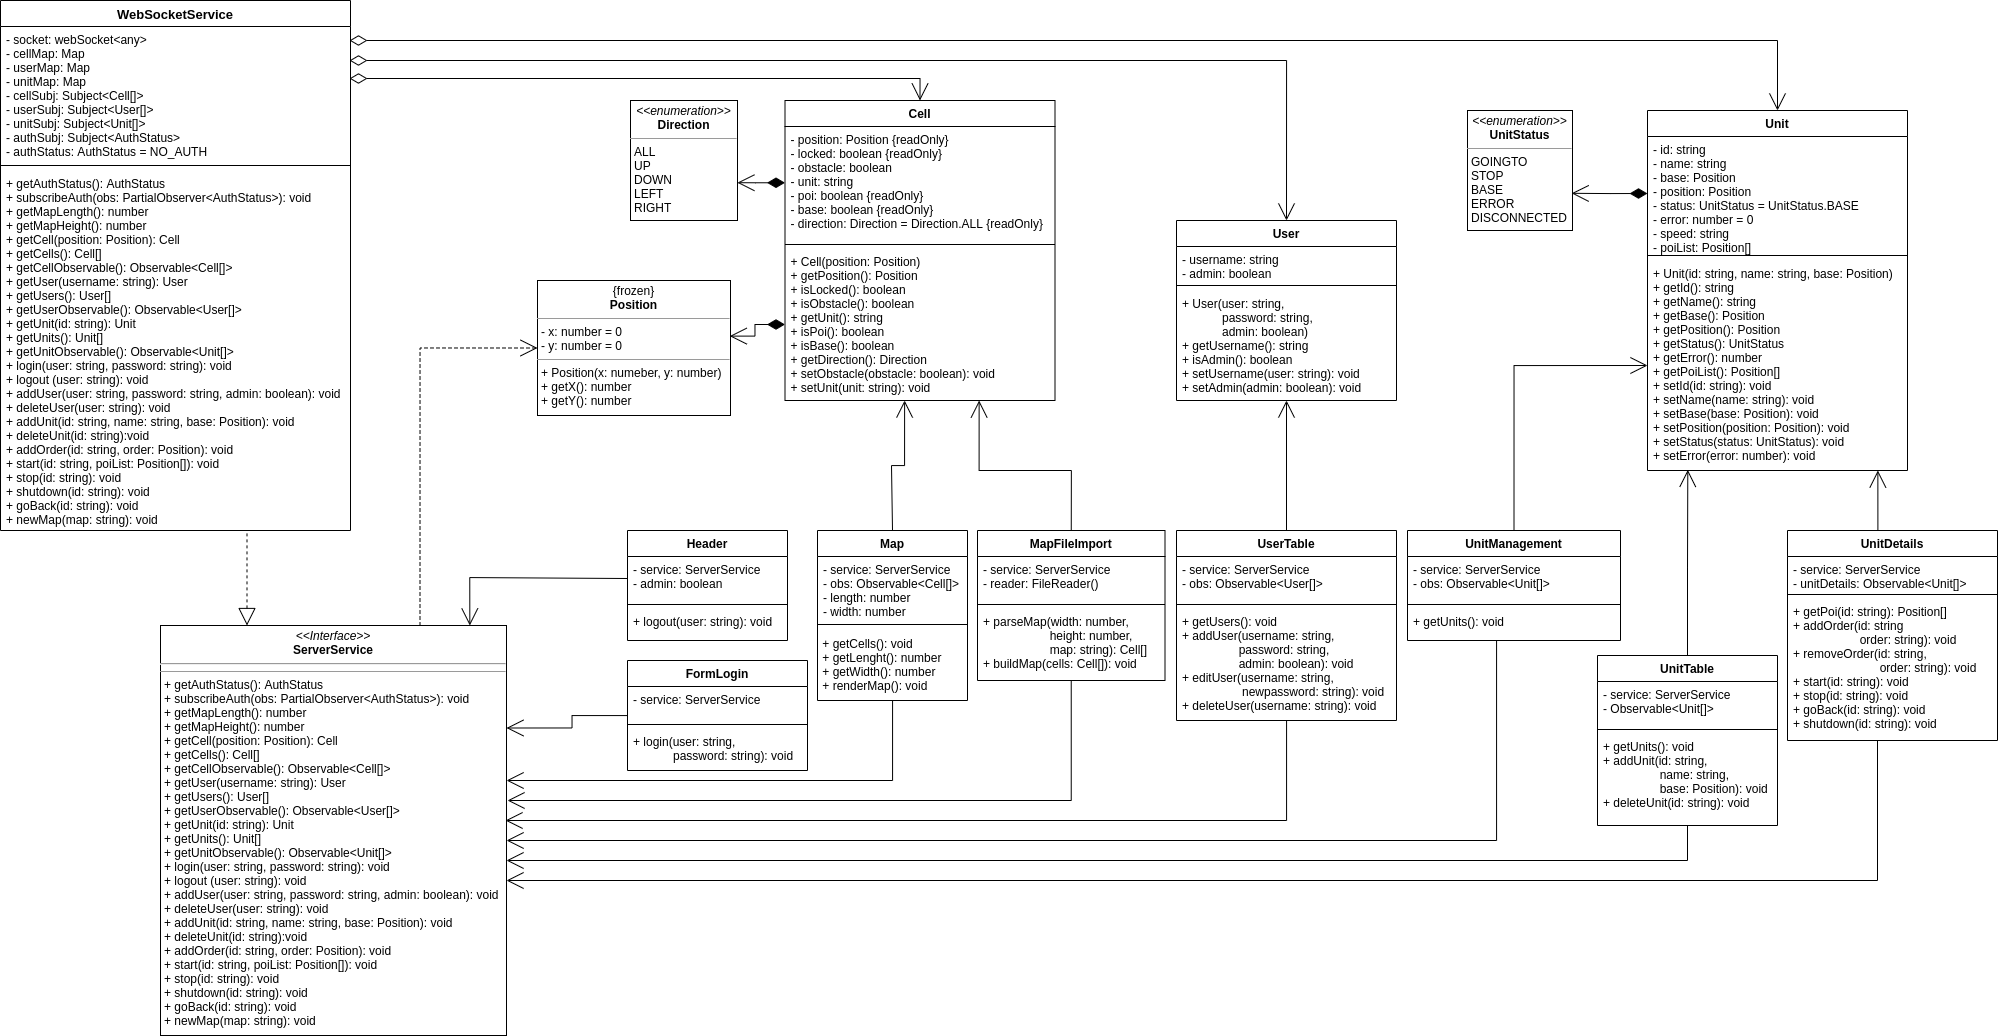
\includegraphics[width=24cm]{img/ui_component.png}
			\caption{Architettura dell'interfaccia - Model-View Model}
		\end{figure}
	\end{landscape}
	\newpage
	
	\begin{landscape}
		\begin{figure}[h!]
			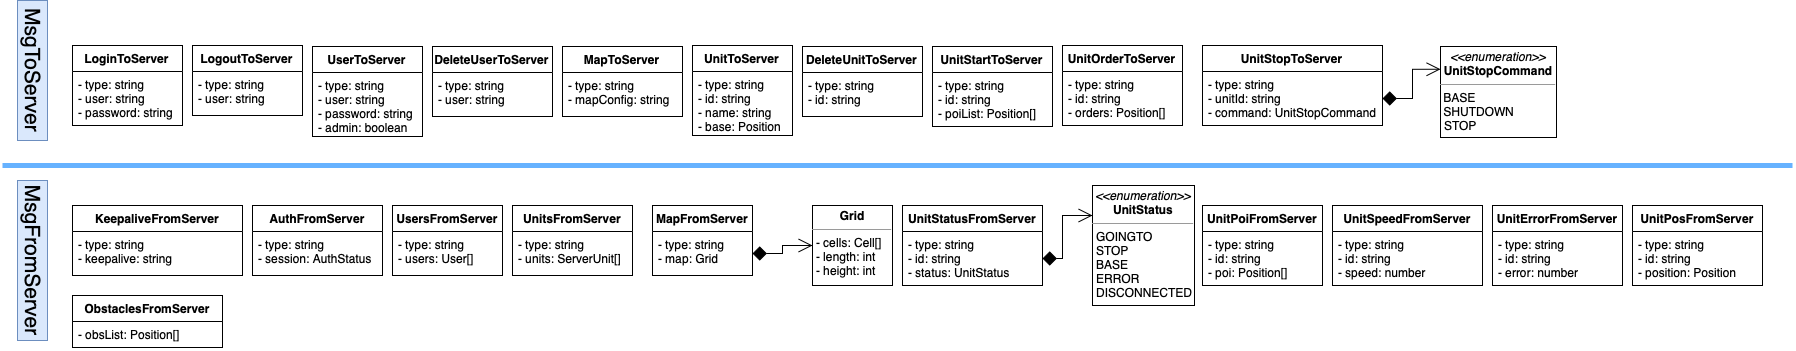
\includegraphics[width=24cm]{img/ui_messaggi.png}
			\caption{Architettura dell'interfaccia - Messaggi}
		\end{figure}
	\end{landscape}

\subsection{Architettura delle unità}
	La componente relativa all'unità viene sviluppata utilizzando il run-time \glock{Node.JS} e i \glock{WebSocket} per la comunicazione con le componenti del server e dei sensori, mentre per lo strato di persistenza si è deciso di fare utilizzo del database \glock{MongoDB}.
	La scelta architetturale per questa componente è ricaduta sulla \textit{Hexagonal Architecture}.
	I motivi riconducibili alla suddetta scelta sono da riscontrarsi nella natura semplicistica del servizio che la componente mette a disposizione. Le logiche di business si occupano unicamente di controllare che i dati ricevuti (già validati nel formato) vengano esaminati e processati per poi essere salvati sul persistence layer.
	Il punto fondamentale è che, oltre ai controller, anche la classe \textit{UnitEngine} si occupa di scrivere e leggere dati dallo strato di persistenza, in modo da emulare l'evolvere degli stati mano a mano che l'unità avanza lungo il percorso e/o incontra ostacoli.
	È inoltre prevista, similmente a quanto accade per la parte relativa alla UI, una gerarchia di interfacce e classi che si occupano di modellare tutti i possibili messaggi che l'unità può voler scambiare con le altre componenti, in modo da controllare in maniera più pulita il passaggio di informazioni.
	Per quanto concerne i sensori, invece, essi non sono dotati di una reale architettura, data la trivialità del loro scopo e del modo in cui il componente opera per raggiungerlo.
	
	\begin{figure}[H]
		\centering
		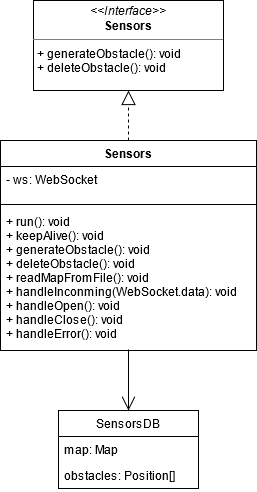
\includegraphics[width=6cm]{img/unit_sensori.png}
		\caption{Unità - Sensori}
	\end{figure}
	
	Di seguito si illustrano i diagrammi delle classi dell'architettura dell'unità, e dei messaggi usati per interfacciarsi con il server.
	
	\begin{landscape}
		\begin{figure}[h!]
			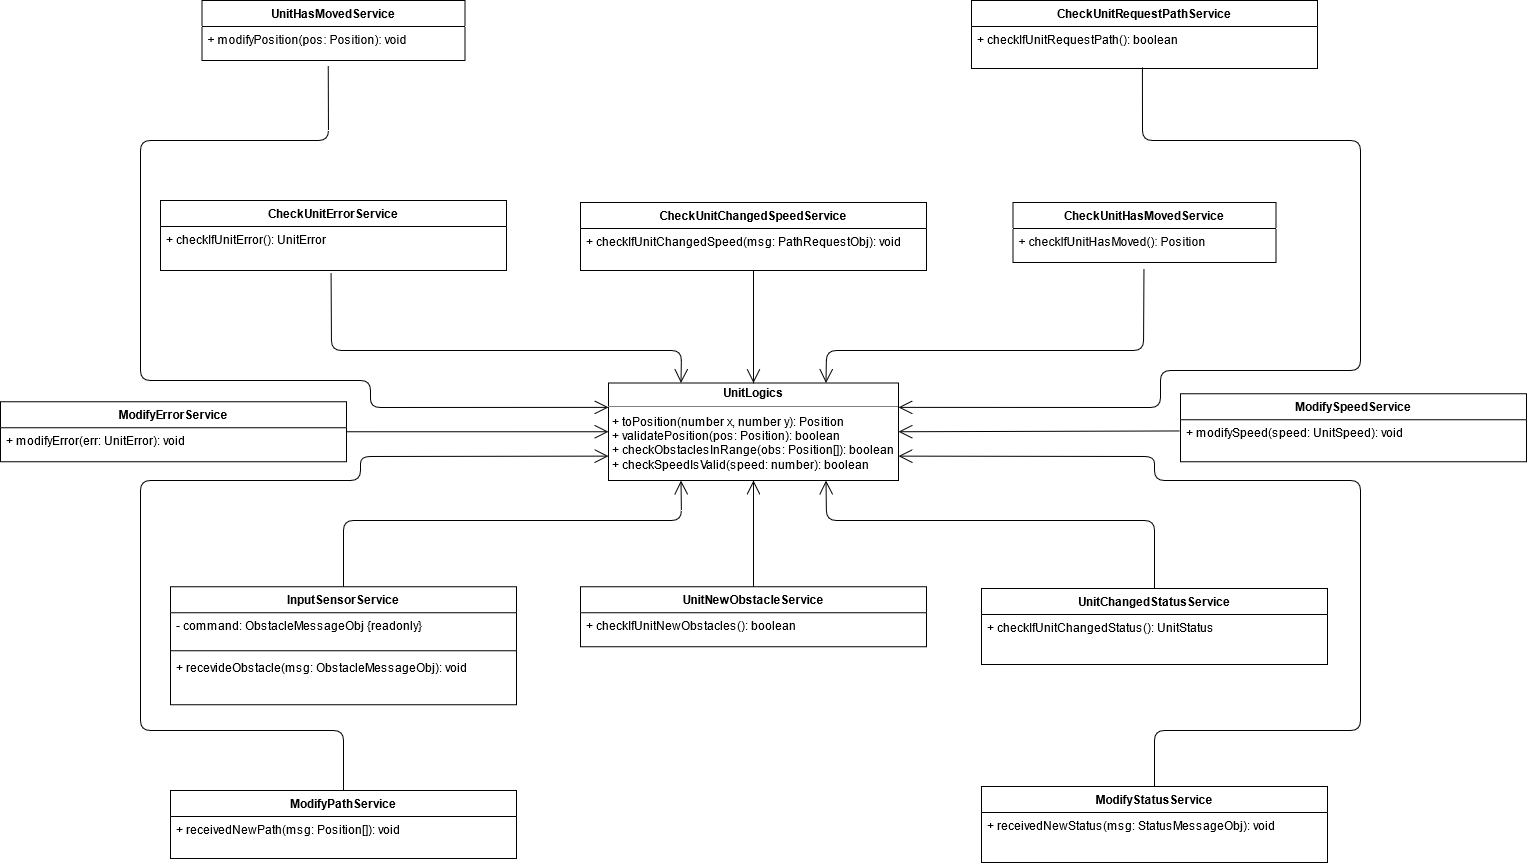
\includegraphics[width=25.5cm]{img/unit_architettura1.png}
			\caption{Unità - Diagramma delle classi}
		\end{figure}
	\end{landscape}
	
	\begin{landscape}
		\begin{figure}[h!]
			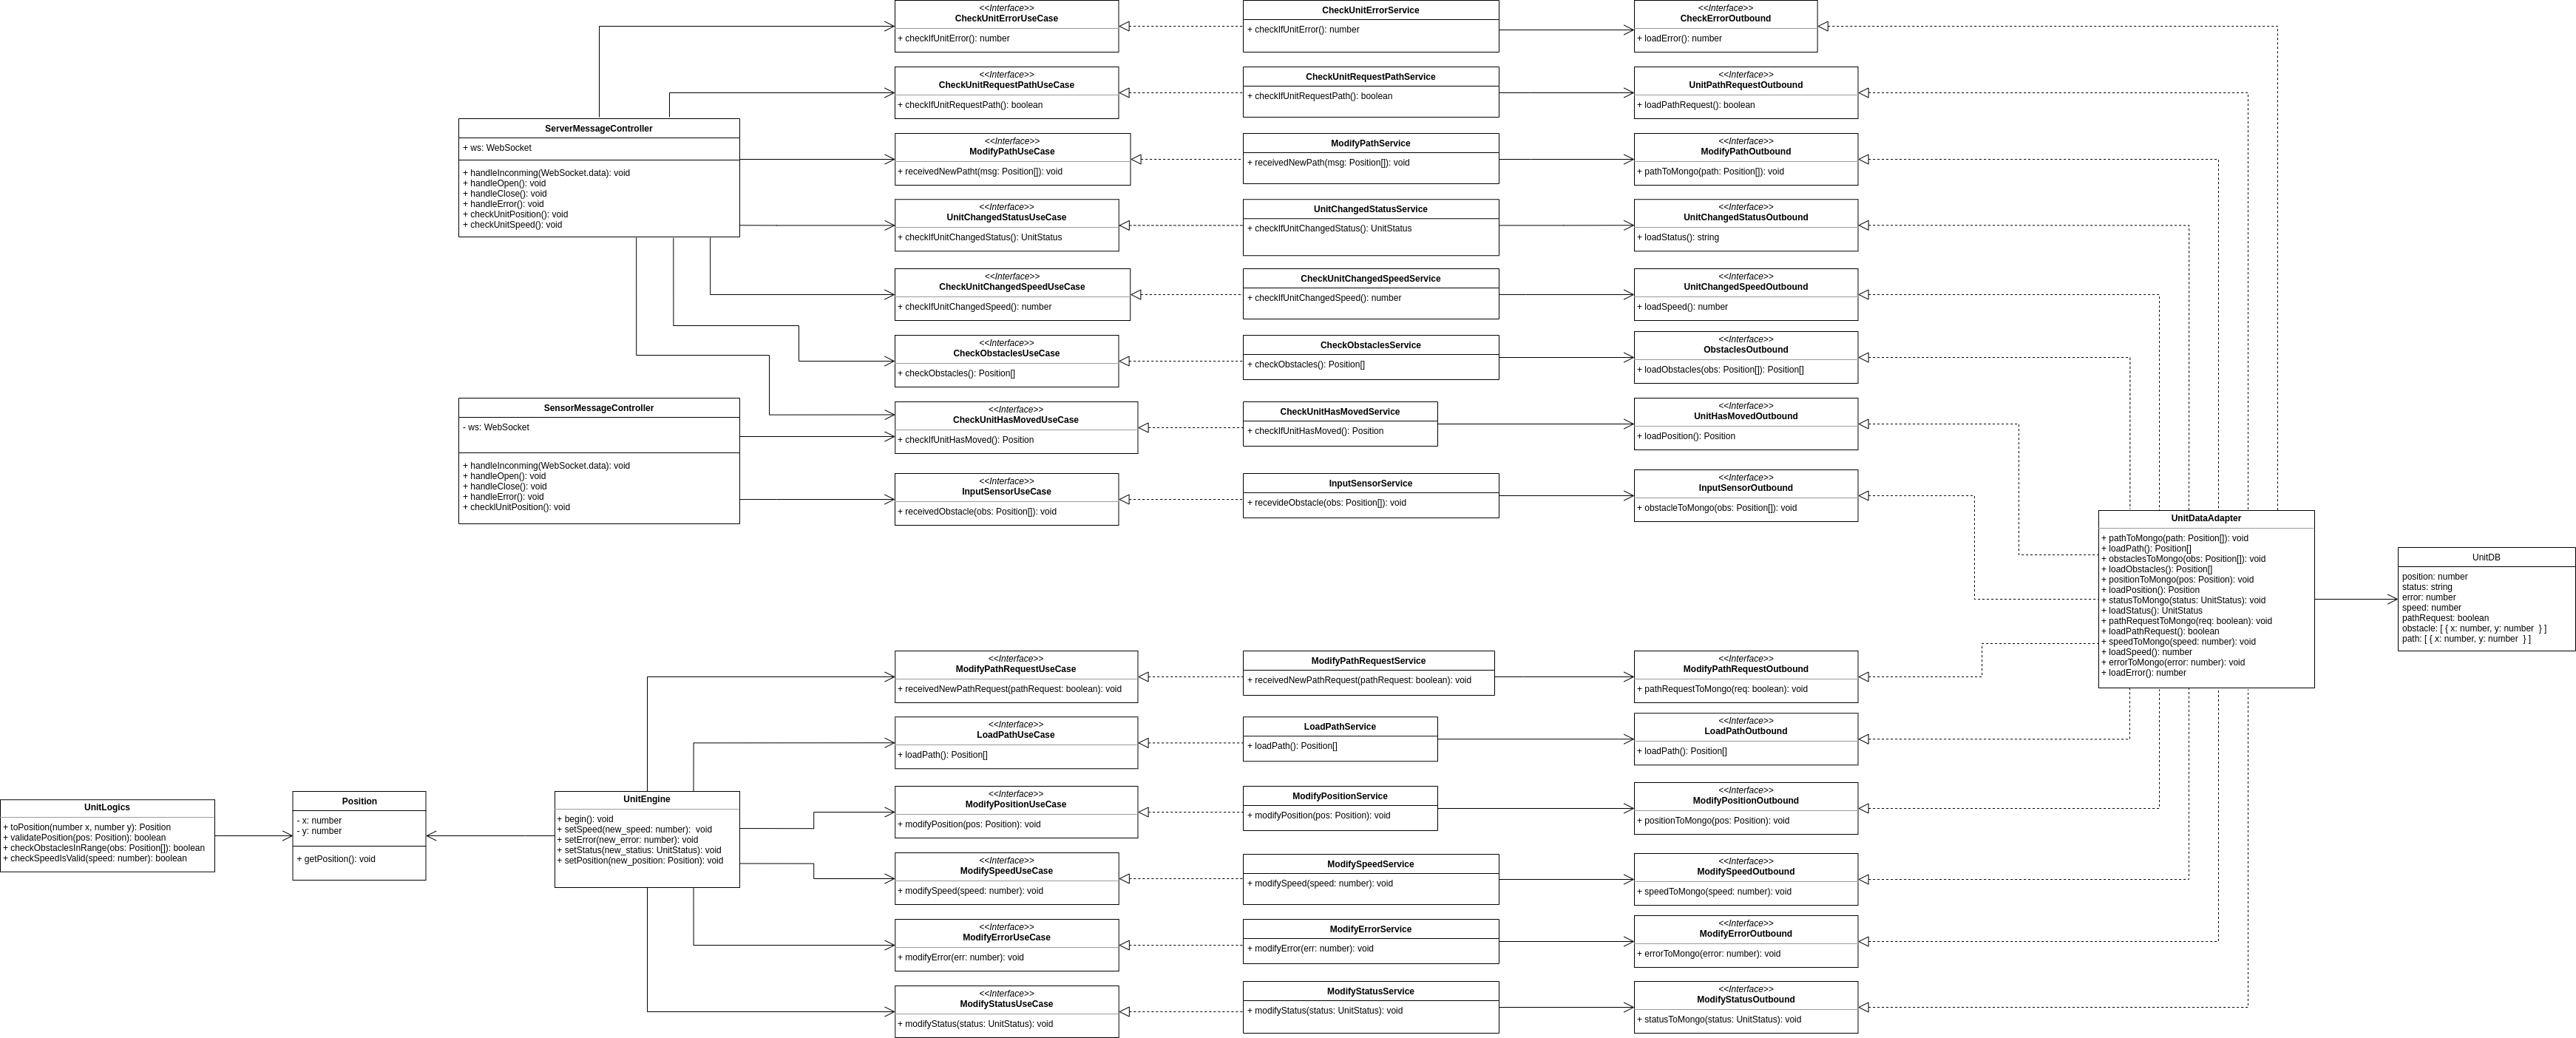
\includegraphics[width=25.5cm]{img/unit_architettura2.png}
			\caption{Unità - Diagramma delle classi}
		\end{figure}
	\end{landscape}
	
	
	\begin{landscape}
		\begin{figure}[H]
			\centering
			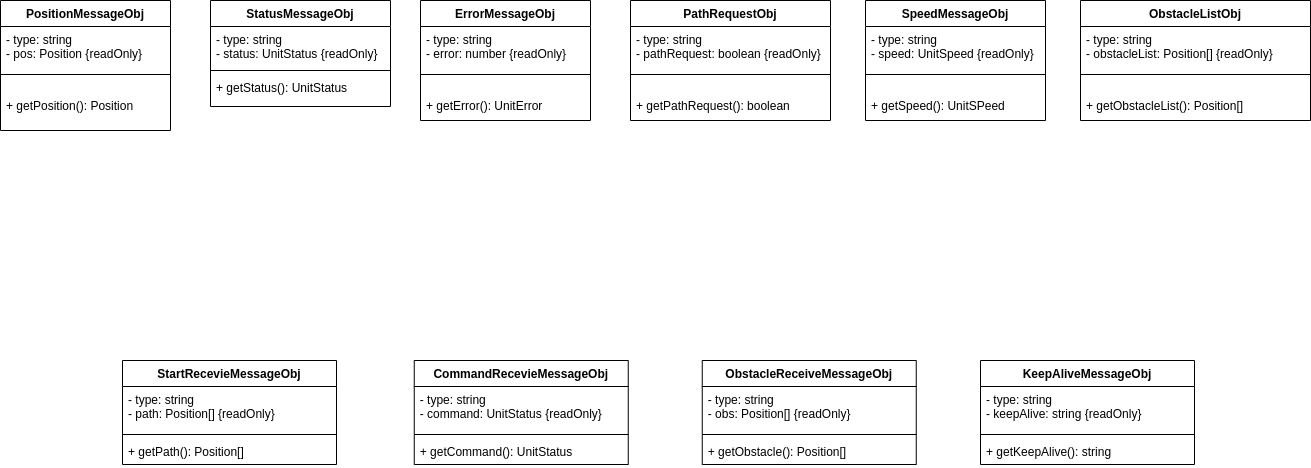
\includegraphics[width=25.5cm]{img/unit_messaggi.png}
			\caption{Unità - Messaggi}
		\end{figure}
	\end{landscape}